\chapter{Electrodin'amica}

\section{Ley de inducci'on de Faraday}

Faraday\footnote{Michael Faraday (1791-1867): f'isico y qu'imico brit'anico. Ver \url{http://es.wikipedia.org/wiki/Michael_Faraday}.} encontr'o experimentalmente (1831) que \textit{si el flujo magn'etico a trav'es de una espira cerrada var'ia en el tiempo, se induce una corriente sobre una espira}. Si el flujo es constante, se observa que la corriente desaparece. La \textbf{ley de Faraday} se escribe como
\begin{equation}\label{faraday}
\varepsilon_{\rm ind}=-K\frac{d\phi}{dt},
\end{equation}
donde $\varepsilon_{\rm ind}$ es la fuerza electromotriz (f.e.m.) \textit{inducida} en la espira. El signo menos describe la direcci'on de la corriente inducida, dada por la \textbf{ley de Lenz}. Aqu'i $K$ es una constante que depende del sistema de unidades usado. En el Sistema Internacional es una cantidad adimensional, que determinaremos m'as adelante.

En t'erminos de campos, se genera un campo el'ectrico $\vec{E}$ que es el que hace mover las cargas en la espira, es decir,
\begin{equation}
\oint_{\cal\partial S}\vec{E}\cdot d\vec{\ell}=\varepsilon_{\rm ind}.
\end{equation}
Con esto, podemos escribir (\ref{faraday}) como
\begin{equation}
\oint_{\cal \partial S}\vec{E}\cdot d\vec{\ell}=-K\frac{d\ }{dt}\int_S\vec{B}\cdot
d\vec{S}.
\end{equation}
En general, la superficie puede variar en el tiempo. Si 'este \textit{no} es el caso, y $S$
es constante, entonces podemos deducir que
\begin{equation}\label{ley-faraday0}
\vec\nabla\times\vec{E}=-K\frac{\partial\vec{B}}{\partial t}.
\end{equation}
Considere ahora el caso en que la espira se mueve \textit{r'igidamente}, es decir, que la velocidad de los puntos de la espira es independiente de la posici'on (puede, sin embargo, depender del tiempo).
Entonces el cambio del flujo por la superficie, entre los tiempos $t$ y $t+dt$, puede calcularse como sigue:
\begin{eqnarray}
 d\Phi &=& \Phi(t+dt)-\Phi(t)\\
&=&
\int_{S(t+dt)}B_i(\vec{x}+\vec{v}dt,t+dt)dS_i-\int_{S(t)}B_i(\vec{x},t)dS_i\\
&=&\int_{S(t+dt)}\left[B_i(\vec{x},t)+dt\,v_j\,\partial_jB_i(\vec{x},
t)+dt\,\partial_tB_i(\vec{x},t)\right ] dS_i-\int_{S(t)}B_i(\vec{x},t)dS_i\\
&=&\int_S\left[B_i(\vec{x},t)+dt\,v_j\,\partial_jB_i(\vec{x},
t)+dt\,\partial_tB_i(\vec{x},t)\right ] dS_i-\int_SB_i(\vec{x},t)dS_i\\
&=&dt\int_S\left[v_j\,\partial_jB_i(\vec{x},t)+\partial_tB_i(\vec{x},t)\right
] dS_i.
\end{eqnarray}
En la pen'ultima igualdad usamos el hecho que el elemento de superficie $dS_i$ sobre la superficie $S(t)$ y $S(t+dt)$ son iguales, ya que la superficie se mueve r'igidamente (es decir, con igual velocidad en cada punto). As'i obtenemos que
\begin{equation}\label{dPhidt0}
 \frac{d\Phi}{dt}=\int_S\left[v_j\,\partial_jB_i(\vec{x},t)+\partial_tB_i(\vec
{x},t)\right] dS_i.
\end{equation}
Usamos ahora la identidad
\begin{equation}
\varepsilon_{ijk}\partial_j(\varepsilon_{klm}B_lv_m)\equiv
v_j(\partial_jB_i)-v_i(\partial_jB_j),
\end{equation}
y la ley (\ref{divB}) (que suponemos v'alida incluso en el caso din'amico) para reescribir (\ref{dPhidt0}) como
\begin{eqnarray}
 \frac{d\Phi}{dt}&=&\int_S\left[\partial_tB_i+\varepsilon_{ijk}
\partial_j(\varepsilon_{klm} B_lv_k)\right] dS_i \\
&=& \int_S\partial_tB_i\, dS_i +\oint_{\partial S}\varepsilon_{ijk}
B_jv_k\,dx_i 
\end{eqnarray}
o, en notaci'on vectorial, 
\begin{equation}\label{dFlujodt}
  \frac{d\Phi}{dt}=\int_S\frac{\partial\vec{B}}{\partial
t}\cdot d\vec{S}-\oint_{\partial
S}\left(\vec{v}\times\vec{B}\right)\cdot d\vec{\ell}.
\end{equation}
Apliquemos estos resultados para comparar la descripci'on, respecto a dos sistemas de referencia inerciales (SRI's), del fen'omeno de inducci'on de corriente en una espira debido a la variaci'on de flujo magn'etico. Primero, en el SRI $K$ en el que la espira est'a en reposo y el magneto se mueve tenemos que en cada punto del espacio el campo magn'etico $\vec{B}$ depender'a del tiempo, por lo que se inducir'a un campo el'ectrico de acuerdo a (\ref{ley-faraday0}). Este campo el'ectrico ejercer'a una fuerza $\vec{F}_q=q\vec{E}$ sobre una carga $q$ en la espira, que consideraremos inicialmente en reposo. 

Por otro lado, en un SRI $K'$ con velocidad relativa $\vec{v}$ respecto a $K$ (de modo que en $K'$ el magneto est'a en reposo) la corriente inducida es debido al movimiento de la espira. Si en este SRI el campo magn'etico es $\vec{B}'(x)$, no existe campo el'ectrico inducido puesto que $\partial\vec{B}'/\partial t=\vec{0}$. En este SRI la corriente inducida se describe 'integramente debido a la fuerza de Lorentz ejercida por el campo magn'etico sobre las cargas en la espira, que ahora se mueven con velocidad $-\vec{v}$. La fuerza que act'ua sobre la carga es ahora $\vec{F}'_q=-q\vec{v}\times\vec{B'}$. Adem'as, la f.e.m. est'a dada, usando el resultado (\ref{dFlujodt}) aplicado a este caso, as'i como la ley de Faraday (\ref{ley-faraday0}), por 
\begin{equation}
\varepsilon'_{\rm ind}=-K\oint_{\partial S}\left(\vec{v}\times\vec{B}'\right)\cdot d\vec{\ell}.
\end{equation}

 Ya que $K$ y $K'$ son SRI's, la aceleraci'on, y por tanto la fuerza que act'ua sobre la carga (inicialmente en reposo en $K$), son necesariamente iguales. De lo anterior, es decir $\vec{F}_q=\vec{F}'_q$, vemos que esto s'olo es posible si el campo inducido es dado por
 \begin{equation}\label{EvBp}
\vec{E}=-\vec{v}\times\vec{B'}.
\end{equation}
Adem'as, la f.e.m. debe ser la misma, ya que la corriente inducida lo es, por lo que
\begin{align}
\varepsilon_{\rm ind} &= \varepsilon'_{\rm ind}, \\
\oint_{\partial S}\vec{E}\cdot d\vec{\ell} &=-K\oint_{\partial S}\left(\vec{v}\times\vec{B}'\right)\cdot d\vec{\ell}.
\end{align}
Usando ahora (\ref{EvBp}) en el lado izquierdo obtenemos
\begin{equation}
-\oint_{\partial S}\left(\vec{v}\times\vec{B'}\right)\cdot d\vec{\ell} =-K\oint_{\partial S}\left(\vec{v}\times\vec{B}'\right)\cdot d\vec{\ell}.
\end{equation}
Esta relaci'on implica que la constante $K$ debe tener, en el Sistema Internacional de Unidades, el valor $K=1$. 

De esta forma, la ley de Faraday adopta la forma
\begin{equation}
\boxed{\oint_{\cal\partial S}\vec{E}\cdot d\vec{\ell}=-\frac{d\ }{dt}\int_S\vec{B}\cdot
d\vec{S}}
\end{equation}
o, en forma diferencial:
\begin{equation}
\boxed{\vec\nabla\times\vec{E}=-\frac{\partial\vec{B}}{\partial t}.}
\label{ley-faraday}
\end{equation}

%\subsection{Autoinducci'on}
%\begin{equation}
% L:=\frac{d\Phi}{dI}
%\end{equation}
%\begin{equation}
% \varepsilon_{\rm ind}=-L\frac{dI}{dt}
%\end{equation}


\subsection{Energ'ia del campo magn'etico}

Consideremos ahora una espira por la que circula una corriente $I$ y el campo magn'etico \textit{que ella misma produce}. Si $I$ no var'ia en el tiempo, no existe fem inducida ya que el flujo magn'etico por la espira permanece constante (suponemos una espira fija, en reposo). Calcularemos la energ'ia necesaria para cambiar la corriente $I$ y el correspondiente campo magn'etico $\vec{B}$ en una peque\~na cantidad. Durante el intervalo de tiempo $dt$ en que la corriente cambia en $dI$ y el campo magn'etico en $d\vec{B}$, se genera un campo el'ectrico inducido y su correspondiente fem $\varepsilon$ (que en general se superponen al campo y fem que mantien'ian la corriente $I$ fluyendo originalmente). Este campo inducido ``intenta reducir'' el cambio de la corriente. Para esto, el campo realiza trabajo sobre las cargas en movimiento en la espira. 
%Calcularemos la energ'ia transferida a las cargas que se ponen en movimiento para formar la corriente inducida en una espira, debido a la inducci'on de Faraday. Para esto, consideraremos una espira que forma una curva cerrada $\cal C$ por la que circula una corriente inducida $I$. 

Dividiremos la curva en elementos de longitud $d\vec{\ell}=d\ell \,\hat{t}$, en los que existe una carga $dq=\lambda d\ell$. El vector unitario $\hat{t}$ est'a definido de modo que $d\vec{\ell}$ tiene la orientaci'on standard respecto al vector normal $\hat{n}$ a la superficie que encierra la espira. El campo el'ectrico $\vec{E}$ ejerce trabajo sobre las cargas $dq$. En un intervalo de tiempo $dt$ el trabajo realizado sobre las cargas $dq$ es entonces 
\begin{align}
dq\,\vec{E}\cdot d\vec{\ell} &= (\lambda d\ell) \vec{E}\cdot (\vec{v}\,dt) \\
&= (\lambda d\ell) \vec{E}\cdot (v\,\hat{t})\,dt \\
&= (\lambda v) \vec{E}\cdot (d\ell\,\hat{t})\,dt \\
&= I(\vec{E}\cdot d\vec{\ell})\,dt.
\end{align}
Aqu'i hemos identificado la corriente $I=\lambda v$ sobre la espira, y tomado en cuenta que $\vec{v}=v\hat{t}$. Por lo tanto, el trabajo total realizado por el campo sobre las cargas de la espira, en el intervalo de tiempo $dt$, es dado por
\begin{align}
dW &= \oint_{\cal C}dq\,\vec{E}\cdot d\vec{\ell} \\
&= I\oint_{\cal C}(\vec{E}\cdot d\vec{\ell})\,dt \\
&= I\varepsilon\,dt \\
&= -I\frac{d\Phi}{dt}\,dt \\
&= -I\,d\Phi.
\end{align}

A partir de este resultado vemos que la energ'ia (proveniente de fuentes externas) necesaria para cambiar el flujo magn'etico en una cantidad $d\Phi$, en un sistema con una corriente $I$ es dada por
\begin{equation}\label{dWIdP}
 \boxed{dU=I\,d\Phi.}
\end{equation}
En otras palabras, \textit{un cambio en el valor de la intensidad de campo $\vec{B}$ requiere invertir energ'ia}. En cierto sentido, la ley de Faraday establece una cierta ``inercia'' en el campo magn'etico, ya que un sistema de cargas y campos tiende a ``resistirse'' al cambio del valor del campo (y su flujo). 
Esto implica adem'as que \textit{es necesario asociar una energ'ia a una cierta configuraci'on de campos y corrientes}, puesto que es necesario invertir energ'ia para establecer estas corrientes y sus campos asociados. Para evaluar esta energ'ia, reescribiremos (\ref{dWIdP}) usando (\ref{PAdx}): la energ'ia $\delta U$ necesaria para variar el potencial vectorial $\vec{A}(x)$ de un sistema de corrientes y campo magn'etico en $\delta\vec{A}(x)$ es dada por
\begin{align}
 \delta U &= I\oint_{\cal C}\delta\vec{A}\cdot d\vec{\ell} \\
 &= \oint_{\cal C}\delta\vec{A}\cdot Id\vec{\ell} \\
 &= \int_V\delta\vec{A}\cdot \vec{J}_{\rm ext}\,dV. \label{WdAJ}
\end{align}
En el 'ultimo paso hemos usado la relaci'on (\ref{IdxJdV}) para reescribir la energ'ia en t'erminos de una integral de volumen de la densidad de corriente. Note que la corriente inducida es en general corriente ``externa'' o de ``conducci'on'', por lo que hemos explicitado en el 'ultimo t'ermino la densidad de corrientes externas $\vec{J}_{\rm ext}$. Adem'as, usando la ley de Amp\`ere para la excitaci'on magn'etica (\ref{rotHj}), podemos escribir
\begin{align}
 \delta U 
&= \int_{V'} \delta A_i\,\varepsilon_{ijk}\left(\partial_jH_k\right)\,dV \\
&= \varepsilon_{ijk}\int_{V'} \left[\partial_j(H_k\delta A_i)-H_k(\partial_j\delta A_i)\right]dV\\
&= \varepsilon_{ijk}\oint_{\partial V'}H_k\delta
A_i\,dS_j-\varepsilon_{ijk}\int_{V'}H_k(\partial_j\delta A_i)\,dV\\
&= 0+\int_{V'} H_k\,\varepsilon_{kji}(\partial_j\delta A_i)\,dV\\
&= \int_{V'} H_k\,\delta B_k\,dV.
\end{align}
Aqu'i hemos extendido el dominio de integraci'on a un volumen $V'\to R_3$, es decir, a todo el espacio, usado el teorema de Gauss y considerado que la integral de superficie se anula en el infinito. Con esto, obtenemos la siguiente expresi'on para la \textit{energ'ia requerida para cambiar la inducci'on magn'etica de un sistema en $\delta{\vec B}(x)$}:
\begin{equation}
 \boxed{\delta U=\int_{R^3} \vec{H}(x)\cdot \delta\vec{B}(x)\,dV.}\label{dUB}
\end{equation}
Note la similitud entre las expresiones (\ref{WdAJ}) y (\ref{dUB}) con los resultados (\ref{Wdiel1}) y (\ref{dUE}) para la energ'ia almacenada por un campo el'ectrico, respectivamente.

*** Agregar comentario energ'ia y 'area bajo la curva de gr'afico $H$ v/s $B$ ***

Similarmente a lo discutido en el caso el'ectrico, la \textit{energ'ia total requerida para aumentar el campo magn'etico de un sistema desde cero hasta un valor final $\vec{B}$} es 
\begin{equation}
 U=\int_0^1\int_{R^3} \lambda \, \vec{H}(x)\cdot \delta\vec{B}_\lambda(x)\,dV,
\end{equation}
donde $\vec{B}_\lambda(x)$ es el valor de la inducci'on magn'etica correspondiente al caso en que la excitaci'on magn'etica tiene un valor $\vec{H}_\lambda(x)$ igual a una fracci'on $\lambda$ de la excitaci'on magn'etica final, es decir, $\vec{H}_\lambda (x)=\lambda\vec{H}_\lambda (x)$ .

En el caso de un \textit{medio magn'etico lineal}, tendremos que $\vec{B}_\lambda (x)=\lambda\, \vec{B}(x)$ y por lo tanto $\delta\vec{B}_\lambda (x)=d\lambda\,
\vec{B}(x)$, y entonces
\begin{equation}\label{UHB}
 \boxed{U=\frac{1}{2}\int_{R^3} \vec{H}(x)\cdot\vec{B}(x)\,dV }
\end{equation}
o, alternativamente, 
\begin{equation}
 \boxed{U=\frac{1}{2}\int_{R^3} \vec{A}\cdot \vec{J}\,dV.}
\end{equation}

Usando (\ref{UHB}) podemos escribir la energ'ia almacenada en un sistema de campo magn'etico (y corrientes) como la integral de una \textbf{densidad de energ'ia magn'etica}
\begin{equation}
 \boxed{U=\int_{R^3} u_B(x)\,dV, \qquad u_B(x):=\frac{1}{2}\vec{H}(x)\cdot\vec{B}(x).}
\end{equation}
En el caso particular de medio lineales e is'otropos la densidad de energ'ia magn'etica se reduce a
\begin{equation}
 u_B(x)=\frac{\mu}{2}\vec{H}^2(x)=\frac{1}{2\mu}\vec{B}^2(x).
\end{equation}


\subsection{Fuerzas y torques sobre circuitos magn'eticos}
%\begin{equation}
%\boxed{F_i=-\left(\frac{\partial U}{\partial x_i}\right) ,} \label{FQB}
%\end{equation}
%
%\begin{equation}
% \boxed{\vec{\tau}\cdot\hat{n}=-\left(\frac{\partial U}{\partial\theta}\right).}
%\end{equation}

\section{Ecuaciones de Maxwell}
Hasta el momento,
\begin{align}
\vec\nabla\cdot\vec{D} & =\rho ,\label{cmax1}\\
\vec\nabla\cdot\vec{B}  & =0 ,\label{cmax2}\\
\vec\nabla\times\vec{H}  & =\vec{J} ,\label{cmax3}\\
\vec\nabla\times\vec{E}  & =-\frac{\partial\vec{B}}{\partial t} .\label{cmax4}
\end{align}
Note que aqu'i hemos suprimido, para no recargar la notaci'on, la designaci'on ``${\rm ext}$'' en la densidad de carga y corriente externa.

Vemos que (\ref{cmax3}) implica $\vec\nabla\cdot\vec{J}=0$, que es una condici'on que \textit{no es v'alida en general}, sino que s'olo en los casos, de acuerdo a (\ref{eccont}), en que ${\partial\rho}/{\partial t}=0$. Esto lleva a pensar que (al menos) la ecuaci'on (\ref{cmax3}) no es v'alida en el caso din'amico m'as general en el que las densidades de carga y corriente, y por lo tanto los campos el'ectricos y magn'eticos, var'ian en el tiempo.

Maxwell\footnote{James Clerk Maxwell (1831-1879): F'isico escoc'es. Ver \url{http://es.wikipedia.org/wiki/James_Clerk_Maxwell}.} (1861) generaliz'o la ecuaci'on (\ref{cmax3}) de modo que sea compatible con (\ref{cmax1}) y la ley de conservaci'on de la carga el'ectrica,
es decir, con la ecuaci'on de continuidad (\ref{eccont}). Usando (\ref{cmax1}), que suponemos por tanto v'alida en el caso general, podemos escribir (\ref{eccont}) como
\begin{eqnarray}
 0&=&\frac{\partial\rho}{\partial t}+\vec{\nabla}\cdot\vec{J}\\
&=& \frac{\partial\ }{\partial
t}\left(\vec\nabla\cdot\vec{D}\right)+\vec{\nabla}\cdot\vec{J}\\
&=& \vec\nabla\cdot\left[\frac{\partial\vec{D}}{\partial t}
+\vec{J}\right].
\end{eqnarray}
De aqu'i vemos que en el caso de corrientes generales (no-est'aticas), $\vec{J}$ tiene divergencia no nula, pero la combinaci'on $\vec{J}+{\partial\vec{D}}/{\partial t}$ \textit{siempre tiene divergencia nula}. A partir de esta observaci'on, Maxwell \textit{postul'o} que el lado derecho de la ecuaci'on (\ref{cmax3}) deb'ia ser reemplazada por la combinaci'on $\vec{J}+{\partial\vec{D}}/{\partial t}$. En otras palabras, Maxwell postul'o que a la densidad de corriente deber'ia agregarse el t'ermino ${\partial\vec{D}}/{\partial t}$, llamado \textit{corriente de desplazamiento}.

Con esto, las ecuaciones de Maxwell adoptan la forma:
\begin{align}
\vec\nabla\cdot\vec{D} & =\rho ,\label{max1}\\
\vec\nabla\cdot\vec{B}  & =0 ,\label{max2}\\
\vec\nabla\times\vec{H}  & =\vec{J}+\frac{\partial\vec{D}}{\partial
t} ,\label{max3}\\
\vec\nabla\times\vec{E}  & =-\frac{\partial\vec{B}}{\partial t}.\label{max4}%
\end{align}

Estas ecuaciones son completadas con las relaciones constitutivas entre
$\vec{E}$ y $\vec{D}$, y entre $\vec{B}$ y $\vec{H}$, as'i como con la expresi'on de la (densidad de) fuerza de Lorentz:
\begin{equation}
\vec{f}=\rho\vec{E}+\vec{J}\times\vec{B}.
\end{equation}

\section{Conservaci'on de la energ'ia y Vector de Poynting}\label{sec:energia}
Calculamos el producto escalar de $\vec{E}$ con la ecuaci'on (\ref{max3}).
Usando notaci'on tensorial, obtenemos:
\begin{equation}
 E_i\frac{\partial D_i}{\partial t}
-E_i\,\varepsilon_{ijk}\partial_jH_k+E_iJ_i=0.
\end{equation}
An'alogamente, el producto escalar entre $\vec{H}$ con la ecuaci'on
(\ref{max4}) implica,
\begin{equation}
H_i\frac{\partial B_i}{\partial t} +H_i\varepsilon_{ijk}\partial_jE_k=0.
\end{equation}
Sumando estas ecuaciones, obtenemos
\begin{align}
0 &= E_i\frac{\partial D_i}{\partial t}+H_i\frac{\partial B_i}{\partial t}
-E_i\varepsilon_{ijk}\partial_jH_k+E_iJ_i+H_i\varepsilon
_{ijk}\partial_jE_k\\
 &= E_i\frac{\partial D_i}{\partial t}+H_i\frac{\partial B_i}{\partial
t}+E_iJ_i+\varepsilon_{ijk}\left(H_i\partial_jE_k-E_i\partial_jH_k\right)\\
 &= E_i\frac{\partial D_i}{\partial t}+H_i\frac{\partial B_i}{\partial
t}+E_iJ_i+\varepsilon_{ijk}\left(H_i\partial_jE_k+E_k\partial_jH_i\right)\\
 &= E_i\frac{\partial D_i}{\partial t}+H_i\frac{\partial B_i}{\partial
t}+E_iJ_i+\partial_j(\varepsilon_{jki}E_kH_i).
\end{align}
En resumen, las ecuaciones de Maxwell (\ref{max3}) y (\ref{max4}) implican que
\begin{equation}
\boxed{\vec{E}\cdot\frac{\partial \vec{D}}{\partial
t}+\vec{H}\cdot\frac{\partial\vec{B}}{\partial t}+
\vec\nabla\cdot(\vec{E}\times\vec{H})
+\vec{E}\cdot\vec{J}=0.} \label{cEem0}
\end{equation}
Es 'util definir el \textit{vector de Poynting}\footnote{John Henry Poynting (1852-1914): f'isico ingl'es. Ver \url{http://es.wikipedia.org/wiki/John_Henry_Poynting} $\leftarrow$ \textbf{Esta p'agina podr'ia ser mejorada considerablemente, traduciendo la correspondiente en ingl'es!. ?`voluntarios?}} como
\begin{equation}\label{defPoy}\marginnote{Vector de Poynting}
\boxed{\vec{S}:=\vec{E}\times\vec{H}.}
\end{equation}
En un peque\~no intervalo de tiempo $dt$ los campos cambian (en cada punto fijo del espacio) en las peque\~nas cantidades dadas por $d\vec{D}=dt\,({\partial \vec{D}}/{\partial t})$ y
$d\vec{B}=dt\,({\partial \vec{B}}/{\partial t})$. Entonces podemos escribir
\begin{equation}
\vec{E}\cdot
d\vec{D}+\vec{H}\cdot d\vec{B}+\vec\nabla\cdot\vec{S}\,dt+\vec{E}\cdot\vec{J}\,
dt=0,
\end{equation}
que, integrado en un volumen $V$ conduce a 
\begin{equation}
\boxed{\int_V\left[\vec{E}\cdot d\vec{D}+\vec{H}\cdot
d\vec{B}\right]dV+\oint_{\partial V}
\vec{S}\cdot d\vec{S}\,dt+\int_V\vec{E}\cdot\vec{J}\,
dVdt=0.} \label{cEem1}
\end{equation}
Identificamos el 'ultimo t'ermino como el \textbf{trabajo realizado por el campo el'ectrico sobre las corrientes}, es decir, la energ'ia transferida del campo a las cargas (o viceversa, dependiendo del signo). Adem'as, de acuerdo a los resultados previos (\ref{dUE}) y (\ref{dUB}) la primera integral puede interpretarse como el \textbf{cambio total de la energ'ia almacenada en forma de campo el'ectrico y magn'etico}, en el volumen $V$. Finalmente, interpretamos la integral de superficie como la \textbf{energ'ia electromagn'etica neta que fluye a trav'es de la superficie $\partial V$}. En otras palabras, interpretamos el vector de Poynting como la \textit{densidad de flujo de energ'ia} electromagn'etica (la energ'ia electromagn'etica transportada por unidad de superficie y unidad de tiempo). De esta forma, (\ref{cEem1}) es una \textit{ecuaci'on de balance (o conservaci'on) de la energ'ia}.

En el caso particular de \textit{medios lineales, no disipativos, y con susceptibilidades
independientes del tiempo}, es decir, tales que
\begin{equation}
D_i=\varepsilon_{ij}E_j, \qquad \partial_t\varepsilon_{ij}=0, \qquad \varepsilon_{ij}=\varepsilon_{ji},
\end{equation}
\begin{equation}
B_i=\mu_{ij}H_j, \qquad \partial_t\mu_{ij}=0, \qquad \mu_{ij}=\mu_{ji},
\end{equation}
podemos reescribir:
\begin{equation}
 \vec{E}\cdot\frac{\partial \vec{D}}{\partial
t}=\frac{1}{2}\frac{\partial\ }{\partial t}\left(\vec{E}\cdot\vec{D}\right),
\qquad
 \vec{H}\cdot\frac{\partial \vec{B}}{\partial
t}=\frac{1}{2}\frac{\partial\ }{\partial t}\left(\vec{H}\cdot\vec{B}\right).
\end{equation}
Con esto, (\ref{cEem0}) es equivalente a
\begin{equation}
\boxed{\frac{\partial u}{\partial
t}+\vec\nabla\cdot\vec{S}+\vec{E}\cdot\vec{J}=0 ,} \label{econtEem}
\end{equation}
donde hemos definido la \textit{densidad de energ'ia del campo
electromagn'etico}:
\begin{equation}\label{uDEHB}
\boxed{u:=\frac{1}{2}\left(\vec{D}\cdot\vec{E}+\vec{H}\cdot\vec{B}\right).}
\end{equation}
La versi'on integral de (\ref{econtEem}) es
\begin{equation}
\frac{d\ }{dt}\left(E_{\rm em}+E_{\rm mec}\right)+\oint_{\partial
V}\vec{S}\cdot d\vec{S}=0 ,
\end{equation}
donde
\begin{equation}
E_{\rm em}=\int_V u\,dV
\end{equation}
es la \textbf{energ'ia electromagn'etica} y, de acuerdo al \textit{teorema de trabajo-energ'ia} \textit{en el caso que no existan otras fuerzas que realicen trabajo sobre las cargas},
\begin{equation}
 \frac{dE_{\rm mec}}{dt}=\int_V\vec{E}\cdot\vec{J}\,dV
\end{equation}
es la variaci'on de energ'ia mec'anica total de las cargas contenidas en $V$.

\section{Conservaci'on del momentum lineal}\label{sec:momentum}
La \textbf{fuerza total que el campo electromagn'etico ejerce sobre las cargas} contenidas en un volumen $V$ es dada por la fuerza de Lorentz:
\begin{equation}
\vec{F}_{\rm em}=\int_V\left(\rho\vec{E}+\vec{J}\times\vec{B}\right)dV .
\end{equation}
Consideremos el integrando de la expresi'on anterior (es decir, la densidad de fuerza) y reemplacemos las fuentes $\rho$ y $\vec{J}$ usando las ecuaciones de Maxwell inhomog'eneas (\ref{max1}) y (\ref{max3}). Con esto, tenemos que
\begin{eqnarray}
f_i&=&\rho E_i+\varepsilon_{ijk}J_jB_k \\
&=&(\partial_jD_j)E_i+\varepsilon_{ijk}(\varepsilon_{
jlm}\partial_lH_m-\partial_tD_j)B_k  \\
&=& \partial_j(D_jE_i)-D_j\partial_jE_i +
(\partial_kH_i)B_k-(\partial_iH_k)B_k-\varepsilon_{ijk}(\partial_tD_j)B_k \\
&=& \partial_j(D_jE_i)-D_j\partial_jE_i +
\partial_k(H_iB_k)-H_i(\partial_kB_k) \nonumber\\
&& -\partial_i(H_kB_k)+H_k(\partial_iB_k)
-\partial_t(\varepsilon_{ijk} D_jB_k)
+\varepsilon_{ijk} D_j(\partial_tB_k) \\
%&=&\partial_j(E_iD_j+H_iB_j-\delta_{ij}H_kB_k)
%-D_j\partial_jE_i+H_j(\partial_iB_j) \nonumber\\
%&& -\partial_t(\varepsilon_{ijk} D_jB_k)
%+\varepsilon_{ijk} D_j(\partial_tB_k) \\
&=&\partial_j(E_iD_j+H_iB_j-\delta_{ij}H_kB_k)
-D_j\partial_jE_i+H_j(\partial_iB_j) \nonumber\\
&& -\partial_t(\varepsilon_{ijk}
D_jB_k)-\varepsilon_{ijk} D_j(\varepsilon_{klm}\partial_lE_m) \\
&=&\partial_j(E_iD_j+H_iB_j-\delta_{ij}H_kB_k)
-D_j\partial_jE_i+H_j(\partial_iB_j) \nonumber\\
&& -\partial_t(\varepsilon_{ijk} D_jB_k)-D_j(\partial_iE_j) +D_j(\partial_jE_i)\\
&=&\partial_j(E_iD_j+H_iB_j-\delta_{ij}H_kB_k)-\partial_t(\varepsilon_{ijk}
D_jB_k)+H_j(\partial_iB_j)- D_j(\partial_iE_j). \label{flc}
\end{eqnarray}
En el caso de medios \textit{lineales, homog'eneos y no disipativos}, es decir, para medios tales que
\begin{equation}
 D_i=\varepsilon_{ij}E_j, \qquad \partial_k\varepsilon_{ij}=0, \qquad \varepsilon_{ij}=\varepsilon_{ji},
\end{equation}
\begin{equation}
 B_i=\mu_{ij}H_j, \qquad \partial_k\mu_{ij}=0,\qquad \mu_{ij}=\mu_{ji},
\end{equation}
podemos escribir
\begin{equation}
 \partial_i(D_jE_j)=\varepsilon_{jk}\partial_i(E_kE_j)=2\varepsilon_{jk}
E_k(\partial_i E_j)=2D_j(\partial_i E_j),
\end{equation}
es decir,
\begin{equation}
 D_j(\partial_i E_j)=\frac{1}{2}\partial_i(D_jE_j). \label{idl1}
\end{equation}
An'alogamente,
\begin{equation}
 H_j(\partial_i B_j)=\frac{1}{2}\partial_i(H_jB_j). \label{idl2}
\end{equation}
Reemplazando (\ref{idl1}) y (\ref{idl2}) en los 'ultimos dos t'erminos de
(\ref{flc}), encontramos
\begin{equation}
 \rho E_i+\varepsilon_{ijk}J_jB_k
=\partial_j\left[E_iD_j+H_iB_j-\frac{1}{2}\delta_{ij}\left(
E_kD_k+H_kB_k\right)\right]-\partial_t(\varepsilon_{ijk}D_jB_k).
\end{equation}
Definimos la \textbf{densidad de momentum} del campo, $\pi_i$, y el \textbf{tensor de tensiones de Maxwell}, $T_{ij}$, por
\begin{equation}
\boxed{\pi_i:=\varepsilon_{ijk}D_jB_k,}
\end{equation}
\begin{equation}
 \boxed{T_{ij}:=\frac{1}{2}\delta_{ij}\left(E_kD_k+B_kH_k\right)-E_iD_j-H_iB_j,}
\end{equation}
y entonces
\begin{equation}
\boxed{f_i+\frac{\partial\pi_i }{\partial t}+\partial_jT_{ij}=0.} \label{lcm}
\end{equation}
Integrando (\ref{lcm}) en un volumen $V$ y usando el teorema de Gauss,
encontramos
\begin{equation}
\boxed{F^{\rm em}_i+\frac{d\ }{dt}P_i^{\rm em}+\oint_{\partial
V}T_{ij}\,dS_j =0,} 
\end{equation}
donde $F^{\rm em}_i$ es la fuerza electromagn'etica total actuando sobre las cargas en $V$, y
\begin{equation}\marginnote{mom. lineal del campo}
 \boxed{P_i^{\rm em}:=\int_V \pi_i\,dV.} \label{defpem}
\end{equation}

Si $\vec{F}_{\rm em}$ coincide con la \textit{fuerza total} sobre las cargas (por ejemplo, si las 'unicas fuerzas involucradas son electromagn'eticas, o si la fuerza neta de origen no electromagn'etico se anula) entonces, usando la \textit{segunda ley de Newton}, tenemos que $\vec{F}_{\rm em}=d\vec{P}_{\rm mec}/dt$, donde $\vec{P}_{\rm mec}$ es el \textbf{momentum lineal total de las cargas} en $V$ (mec'anico). Bajo estas condiciones, podemos escribir
\begin{equation}
\boxed{\frac{d\ }{dt}\left(P_i^{\rm mec}+P_i^{\rm em}\right)+\oint_{\partial
V}T_{ij}\,dS_j =0.} \label{licml}
\end{equation}
En casos en que los campos se anulan en $\partial V$, la relaci'on
(\ref{licml}) expresa que $P_i^{\rm mec}+P_i^{\rm em}$ es conservado. Esto
permite interpretar (\ref{defpem}) como el \textbf{momentum lineal total del
campo electromagn'etico en el volumen} $V$. En el caso general $\oint_{\partial
V}T_{ij}\,dS_j $ representa entonces el \textbf{flujo de momentum por unidad de tiempo
a trav'es de} $\partial S$. Consecuentemente, el tensor de Maxwell $T_{ij}$
representa el momentum en la direcci'on $i$ que se transfiere en la direcci'on
$j$, por unidad de tiempo y 'area. Equivalentemente, $-T_{ij}n_j$ ($dS_j=n_jdS$)
representa la \textit{fuerza por unidad de 'area} (tensi'on) que act'ua sobre el sistema
de cargas y campos en $V$.

La expresi'on (\ref{licml}) puede ser usada para calcular la fuerza que act'ua
sobre cargas en presencia de campos electromagn'eticos. Por ejemplo,

\begin{center}
*** EJEMPLO CONDENSADOR PLACAS PARALELAS ***
\end{center}

\textbf{Para un medio lineal \textit{e is'otropo}, el tensor de Maxwell es sim'etrico
$T_{ij}=T_{ji}$} y la densidad de momentum es proporcional al vector de
Poynting, $\vec{\pi}=\varepsilon\mu\,\vec{S}$, de modo que la direcci'on del
momentum de campo coincide con la del flujo de energ'ia de
'este.

\section{Ondas Electromagn'eticas}

\subsection{Campos electromagn'eticos y ecuaci'on de la onda}

Consideremos un \textit{medio lineal, is'otropo y homog'eneo}. En este caso, a ley de Amp\`ere-Maxwell se reduce a
\begin{equation}
\varepsilon_{ijk}\partial_jB_k=\mu\vec{J}+\varepsilon\mu\frac{\partial E_i}{\partial t}.
\end{equation}
Derivando con respecto al tiempo y usando la ley de Faraday, podemos escribir
\begin{eqnarray}
\mu \frac{\partial J_i}{\partial t}+\varepsilon\mu\frac{\partial^2E_i}{\partial t^2}
&=&\varepsilon_{ijk}\partial_j\frac {\partial B_k}{\partial t} \\
&=&-\varepsilon_{ijk}\partial_j\left(\varepsilon_{klm}\partial_lE_m \right)\\
&=&-\left( \delta_{il}\delta_{jm}-\delta_{im}\delta_{jl}\right)
\partial_j\partial_lE_m\\
&=&\partial_j\partial_jE_i-\partial_j\partial_iE_j.
\end{eqnarray}
Usando la ley de Gauss, $\partial_jE_j=\rho/\varepsilon$ en el segundo t'ermino del lado derecho, obtenemos
\begin{equation}\label{EcOihE}
\boxed{\nabla^2\vec{E}-\varepsilon\mu\frac{\partial^2\vec{E}}{\partial t^2}=\frac{1}{\varepsilon}\vec\nabla\rho+\mu\frac{\partial\vec{J}}{\partial t}.}
\end{equation}

Similarmente, calculando la derivada con respecto al tiempo de la ley de Faraday y usando la ley de Amp\`ere-Maxwell, as'i como el hecho que el campo magn'etico siempre tiene divergencia nula, es decir \eqref{max2}, encontramos que
\begin{equation}\label{EcOihB}
\boxed{\nabla^2\vec{B}-\varepsilon\mu\frac{\partial^2\vec{B}}{\partial t^2}=-\mu\vec\nabla\times\vec{J}.}
\end{equation}

De esta forma encontramos que \textit{las ecuaciones de Maxwell implican que los
campos el'ectrico y magn'etico satisfacen la ecuaci'on de onda inhomog'enea}. Es importante notar que \textit{no todas} las soluciones de la ecuaci'on de onda son necesariamente soluciones de las ecuaciones de Maxwell. En otras palabras, \eqref{EcOihE} y \eqref{EcOihB} son \textit{condiciones necesarias, pero no suficientes} para que los campos satisfagan las ecuaciones de Maxwell.

\textbf{En regiones en libres de cargas y corrientes} \eqref{EcOihE} y \eqref{EcOihB} se reducen a la ecuaci'on de onda homog'enea para cada componente (cartesiana) de los campos el'ectrico y magn'etico:
\begin{equation}\label{econdaE}
\boxed{\nabla^2E_i-\varepsilon\mu\frac{\partial^2E_i}{\partial t^2}=0.}
\end{equation}
\begin{equation}
\boxed{\nabla^2B_i-\varepsilon\mu\frac{\partial^2B_i}{\partial t^2}=0.}
\label{econdaB}
\end{equation}



\subsection{Ondas electromagn'eticas planas monocrom'aticas}
Consideremos una soluci'on de \textit{onda plana monocrom'atica polarizada linealmente}:
\begin{equation}
E_i=E_i^0 \cos\left(\vec{k}\cdot\vec{x}-\omega t+\varphi_0\right)
.\label{ecuc-max-solu1}%
\end{equation}
Reemplazando (\ref{ecuc-max-solu1}) en (\ref{econdaE}) encontramos que%
\begin{equation}
\left(k^2-\varepsilon\mu\,\omega^2\right)  E_i=0, \qquad k:=|\vec{k}|,
\end{equation}
por lo que las soluciones no triviales requieren que se satisfaga la
\textit{relaci'on de dispersi'on}:
\begin{equation}
\omega^2=\frac{1}{\varepsilon\mu}\,k^2, \label{rdoem}
\end{equation}
de donde obtenemos la \textit{velocidad de fase},
$v_{\rm f}:=\omega/k$,
\begin{equation}
v_{\rm f}=\frac{1}{\sqrt{\varepsilon\mu}},
\end{equation}
que adem'as, coincide con la \textit{velocidad de grupo}, 
\begin{equation}
v_{\rm f}=v_{\rm g}=\frac{1}{\sqrt{\varepsilon\mu}}=:c,
\end{equation}
donde $v_{\rm g}:=\partial\omega/\partial k$. Esto implica que las ondas electromagn'eticas se propagan de forma \textit{no-dispersiva} (en medios lineales, is'otropos y homog'eneos). 

La \textit{velocidad de la luz en el medio} ($c$) puede ser escrita en t'erminos de la \textit{velocidad de la luz en el vac'io} ($c_0=1/\sqrt{\varepsilon_0\mu_0}$), la susceptibilidad el'ectrica relativa ($\kappa_{\rm m}$) y la permeabilidad magn'etica relativa ($\kappa_{\rm m}$), es decir, usando $\varepsilon=\kappa\varepsilon_0$ y $\mu=\kappa_{\rm m}\mu_0$:
\begin{equation}
c=\frac{c_0}{\sqrt{\kappa\kappa_{\rm m}}}=\frac{c_0}{n}.
\end{equation}
Aqu'i $n:=\sqrt{\kappa\kappa_{\rm m}}$ es el \textit{'indice de refracci'on del medio}.

Adem'as, usando (\ref{max4}) obtenemos
\begin{equation}\label{BkE}
 \vec{B}=\frac{1}{\omega}\,\vec{k}\times\vec{E}.
\end{equation}
Similarmente, usando (\ref{max3}) encontramos que
\begin{equation}
 \vec{E}=-\frac{1}{\varepsilon\mu}\frac{1}{\omega}\,\vec{k}\times\vec{B}.
\end{equation}

Estas relaciones implican que $\vec{k}$, $\vec{E}$ y $\vec{B}$ son ortogonales
entre s'i y forman (en ese orden) un \textit{sistema derecho}. Como consecuencia, \textbf{una onda electromagn'etica plana es \textit{transversal}}, ya que las oscilaciones (de los campos el'ectrico y magn'etico) se producen en el plano ortogonal a la direcci'on de propagaci'on. Adem'as, los m'odulos de los campos satisfacen
\begin{equation}
 | \vec{E}|=c\,| \vec{B}| .
\end{equation}
\begin{figure}[!h]
\centerline{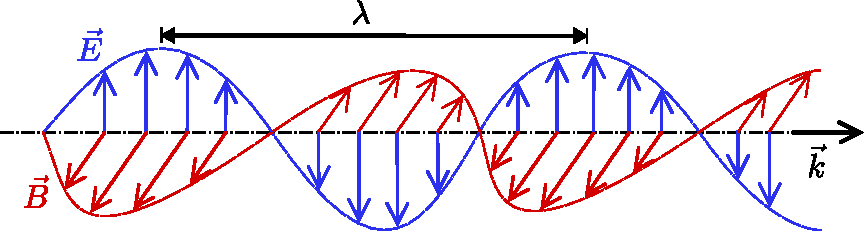
\psfig{file=fig/fig-onda-electromagnetica.pdf,height=3cm,angle=0}}
\caption{Campos el'ectrico y magn'etico de una onda electromagn'etica plana monocrom'atica. Adaptada a partir de \href{http://commons.wikimedia.org/wiki/File:Onde_electromagnetique.svg}{esta} figura original.}
\label{ondaem}
\end{figure}

\subsubsection{Vector de Poynting}
Evaluamos el vector de Poynting (\ref{defPoy}) para la soluci'on de onda plana monocrom'atica reci'en analizada. Usando (\ref{defPoy}), \eqref{BkE} y \eqref{rdoem} podemos escribir
\begin{eqnarray}
 \vec{S}&=&\vec{E}\times\vec{H} \\
&=&\frac{1}{\mu}\,\vec{E}\times\vec{B} \\
&=&\frac{1}{\mu}\,\vec{E}\times\left[\frac{1}{\omega}\,\vec{k}\times\vec{E}
\right] \\
&=&\frac{1}{\mu\omega}\,\vec{E}^2\,\vec{k}\\
&=&\frac{1}{\mu c}\,\vec{E}^2\,\hat{k}. \label{Sop}
\end{eqnarray}
Encontramos de este modo que el campo electromagn'etico correspondiente a la onda plana estudiada \textbf{transporta energ'ia en la direcci'on del vector de onda $\vec{k}$}. Su magnitud, aunque siempre no-negativa, var'ia en el tiempo y con la posici'on, ya que $\vec{E}=\vec{E}(\vec{x},t)$. Como la onda considerada es peri'odica, de periodo $T=2\pi/\omega$, es usual considerar el \textit{promedio del vector de Poynting en un periodo de oscilaci'on}\footnote{Si $f(t)$ es una funci'on del tiempo, entonces definimos su promedio entre $t=0$ y $t=T$ como 
\begin{equation}
\left<f\right>:=\frac{1}{T}\int_0^Tf(t)\,dt.
\end{equation}}
Para la onda sinusoidal (\ref{ecuc-max-solu1}) encontramos entonces que
\begin{equation}\label{Sprom}
\langle\vec{S}\rangle=\frac{1}{2\mu c}\,\vec{E}_0^2\,\hat{k}.
\end{equation}
Esto implica que a trav'es de una superficie de 'area $A$ transversal al vector de onda $\vec{k}$, la onda transporta energ'ia a una tasa (potencia) promedio (en una oscilaci'on) de 
\begin{equation}
 \left<P\right>=\frac{A}{2\mu c}\,\vec{E}_0^2.
\end{equation}

\subsubsection{Densidad de Energ'ia}
An'alogamente, calculamos la densidad de energ'ia electromagn'etica, usando la expresi'on (\ref{uDEHB}):
\begin{eqnarray}
 u&=&\frac{1}{2}\left(\varepsilon\vec{E}^2+\frac{1}{\mu}\vec{B}^2\right)\\
&=&\frac{1}{2}\left(\varepsilon\vec{E}^2+\frac{1}{\mu c^2}\vec{E}^2\right)\\
&=&\frac{1}{2}\left(\varepsilon\vec{E}^2+\varepsilon\vec{E}^2\right)\\
&=&\varepsilon\vec{E}^2. \label{uepE2}
\end{eqnarray}
Similarmente al caso del vector de Poynting, la densidad de energ'ia (siempre no-negativa) var'ia en el tiempo y punto a punto. 
Usando \eqref{uepE2} podemos reescribir el vector de Poynting (\ref{Sop}) como
\begin{equation}
 \vec{S}=u\,c\hat{k}.
\end{equation}
Note que esta expresi'on es an'aloga a $\vec{J}=\rho\vec{v}$ que relaciona la densidad de corriente asociada al movimiento de una densidad $\rho$ (de carga o masa, por ejemplo) con velocidad $\vec{v}$ (``flujo convectivo").

Para la onda peri'odica considerada, podemos calcular la densidad de energ'ia promedio, obteniendo
\begin{equation}\label{uprom}
\left<u\right>=\frac{\varepsilon}{2}\vec{E}_0^2.
\end{equation}

\begin{figure}[!h]
\centerline{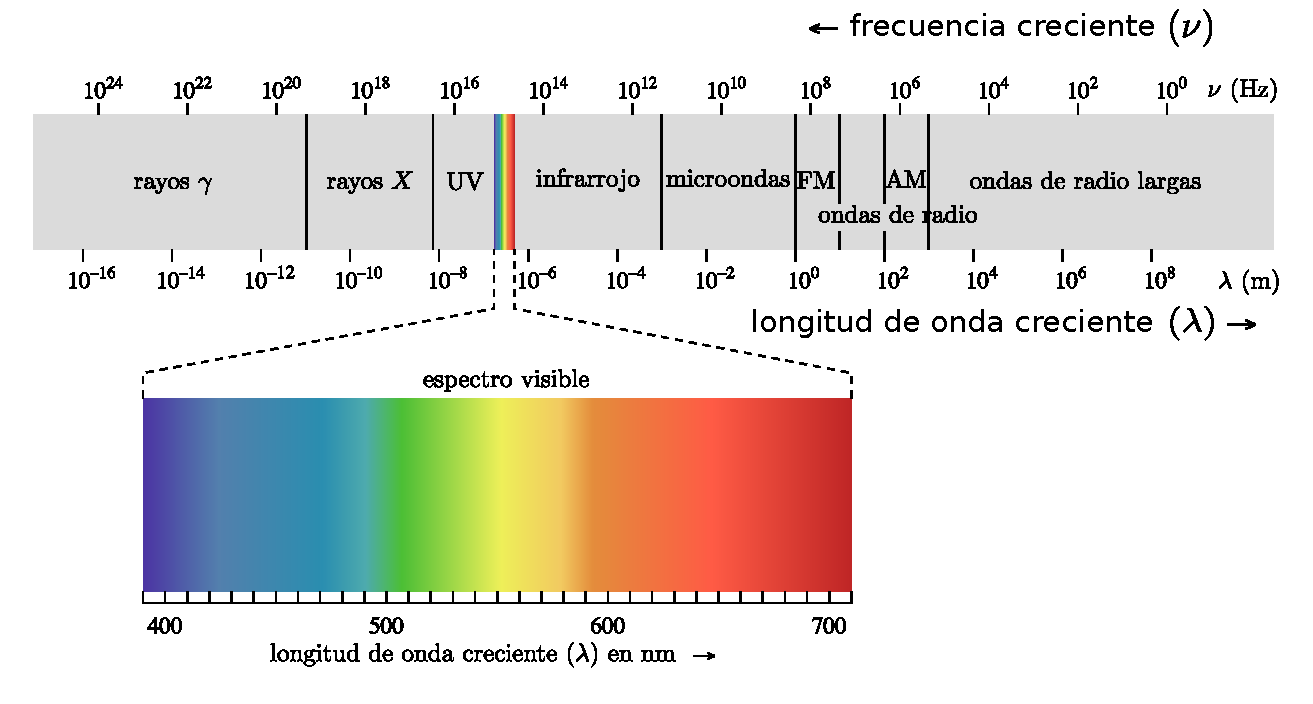
\psfig{file=fig/fig-EM_spectrum_es.pdf,height=7cm,angle=0}}
\caption{Espectro electromagn'etico. Adaptada a partir de \href{http://commons.wikimedia.org/wiki/File:EM_spectrum_es.svg}{esta} figura original.}
\label{fig:EMS}
\end{figure}

\subsection{Ondas electromagn'eticas en la materia}
\subsection{'Indices de reflexi'on y refracci'on}
\subsection{Gu'ias de onda y cavidades resonantes}


\section{Potenciales y transformaciones de gauge}

Las ecuaciones de Maxwell conforman un conjunto de 8 ecuaciones diferenciales
parciales para las 6 componentes del campo electromagn'etico. A menudo es
\textit{conveniente} reducir el n'umero de variables. Esto puede ser conseguido
expresando los campos en t'erminos de \textit{potenciales electromagn'eticos},
de modo que \textit{las ecuaciones homog'eneas de Maxwell sean satisfechas
autom'aticamente} y el n'umero de campos a determinar se reduce a 4. Estos
potenciales se reducen en los casos estacionarios al conocido potencial
electrost'atico y al potencial vectorial magn'etico.

En el caso din'amico general, de (\ref{max2}) podemos concluir que $\vec{B}$
puede ser derivado de un \textit{potencial vectorial}:
\begin{eqnarray}\label{defA2}
\boxed{\vec{B}=\vec{\nabla}\times \vec{A}.}
\end{eqnarray}
Usando esto en (\ref{max4}), obtenemos:
\begin{equation}
\vec{\nabla}\times \vec{E} = -  \frac{\partial\ }{\partial
t}(\vec{\nabla}\times\vec{A}) = -\vec{\nabla}\times
\frac{\partial\vec{A}}{\partial t},
\end{equation}
es decir,
\begin{eqnarray}
\vec{\nabla}\times \left[ \vec{E} + \frac{\partial \vec{A}}{\partial t} \right]
= \vec{0}.
\end{eqnarray}
De aqu'i vemos que el campo vectorial dado por la suma $\vec{E} + {\partial
\vec{A}}/{\partial t}$ puede ser escrito como gradiente de un campo escalar, esto es:
\begin{equation}
\vec{E} + \frac{\partial \vec{A}}{\partial t}= - \vec{\nabla}\phi ,
\end{equation}
de donde
\begin{equation}\label{defphi2}
\boxed{\vec{E} =   - \vec{\nabla}\phi - \frac{\partial \vec{A}}{\partial t}.}
\end{equation}
Las ecuaciones (\ref{defA2}) y (\ref{defphi2}) muestran que el campo
electromagn\'etico puede ser escrito en t\'erminos de un potencial vectorial
$\vec{A}$ y de un potencial escalar $\phi$. Sin embargo, estas funciones
\textit{no son 'unicas} para $\vec{E}$ y $\vec{B}$ dados. Es f\'acil verificar
que el campo electromagn\'etico (y consecuentemente todas las predicciones de la
teor'ia electromag\'etica) permanece invariante (es decir, con igual valor) bajo las
siguientes transformaciones de los potenciales,
\begin{equation}\marginnote{Transformaciones de gauge}\label{tgg}
\boxed{{\vec{A}}' = \vec{A} - \vec{\nabla}{\chi}, \qquad \phi' =\phi +
\frac{\partial \chi}{\partial t},}
\end{equation}
conocidas como \textit{transformaciones de gauge} y donde $\chi=\chi(\vec{x},t)$
es una
funci\'on escalar \textit{arbitraria} del espaciotiempo\footnote{La invariancia
de la teor'ia electromagn\'etica bajo transformaciones de gauge
desempe\~na un rol muy importante. La generalizaci\'on de esta propiedad de
invariancia a \textit{grupos de simetr'ia interna} permiti\'o formular
teor'ias consistentes para las \textit{interacciones d\'ebiles} unificadas con la electromagn\'etica (\textit{electrod\'ebil}) y para la \textit{interacci\'on fuerte}
(\textit{cromodin\'amica cu\'antica}). La \textit{interacci'on gravitacional} tambi\'en puede ser descrita, con algunas peculiaridades, como una \textit{teor'ia de gauge}.}.

\subsubsection{Ecuaciones de Maxwell inhomog'eneas en t'erminos de los
potenciales}
Consideremos el caso de un medio lineal, is'otropo y homog'eneo. Usando (\ref{defA2}) y (\ref{defphi2}) en las ecuaciones inhomog'eneas (\ref{max1}) y (\ref{max3}) encontramos:
\begin{equation}\label{emiap1}
 \nabla^2\phi+\frac{\partial\ }{\partial t}\left(\vec{\nabla}\cdot\vec{A}\right)=-\frac{\rho}{\varepsilon},
\end{equation}
\begin{equation}\label{emiap2}
 \nabla^2\vec{A}-\frac{1}{c^2}\frac{\partial^2\vec{A}}{\partial t^2}-\vec{\nabla}\left(\vec{\nabla}\cdot\vec{A}+\frac{1}{c^2}\frac{\partial\phi }{\partial t}\right)=-\mu\,\vec{J}.
\end{equation}
De esta forma, hemos reducido las ecuaciones de Maxwell a un conjunto de 4 ecuaciones diferenciales parciales para los 4 potenciales. Sin embargo, estas ecuaciones no determinan completamente los potenciales, puesto que las transformaciones de gauge \eqref{tgg} \textit{dejan invariantes} \eqref{emiap1} y \eqref{emiap1}. Esto es natural ya que estas ecuaciones dependen en realidad de los campos el'ectrico y magn'etico, y como vimos las transformaciones de gauge no cambian los valores de estos campos. Adem'as, las ecuaciones \eqref{emiap1} y \eqref{emiap1} est'an \textit{acopladas}, en el sentido que cada una de estas ecuaciones involucra ambos potenciales electromagn'eticos.

Es posible explotar la ``\textit{libertad de gauge}'' de la electrodin'amica (es decir, el hecho que los potenciales no son 'unicos) para \textit{simplificar algunos c'alculos}. Una forma de hacer esto es trabajar con potenciales que satisfagan alguna condici'on extra o \textit{gauge}. De hecho, el imponer condiciones extras a los potenciales no s'olo es conveniente, sino tambi'en \textit{necesario}, ya que las ecuaciones \eqref{emiap1} y \eqref{emiap1} no determinan en forma 'unica los campos $\phi$ y $\vec{A}$. Es posible imponer infinitos gauges diferentes para los potenciales (siempre que sean consistentes con las ecuaciones de Maxwell), pero existen algunos de especial utilidad y popularidad.

\subsubsection{Gauge de Coulomb}
Si el potencial vectorial satisface
\begin{equation}\marginnote{Gauge de Coulomb}\label{gaugeC}
\boxed{ \vec{\nabla}\cdot\vec{A}\stackrel{!}{=}0,}
\end{equation}
se dice que se satisface el \textit{gauge de Coulomb}, \textit{gauge de radiaci'on} o \textit{gauge transversal}. En este caso (\ref{emiap1}) y (\ref{emiap2}) se reducen a
\begin{equation}\label{emiap1GC}
 \nabla^2\phi=-\frac{\rho}{\varepsilon},
\end{equation}
\begin{equation}\label{emiap2GC}
 \nabla^2\vec{A}-\frac{1}{c^2}\frac{\partial^2\vec{A}}{\partial t^2}=-\mu\,\vec{J}+\frac{1}{c^2}\vec{\nabla}\left(\frac{\partial\phi }{\partial t}\right).
\end{equation}

Para probar que \textbf{siempre es posible imponer la condici'on de gauge de Coulomb}, podemos considerar el caso en que inicialmente se trabaje con potenciales $\phi_0$ y $\vec{A}_0$ que no satisfacen la condici'on (\ref{gaugeC}), es decir, $\vec\nabla\cdot\vec{A}_0\neq 0$, y luego demostrar que es posible realizar una transformaci'on de gauge (\ref{tgg}) con una funci'on $\chi$ tal que los nuevos potenciales s'i satisfagan (\ref{gaugeC}). Usando (\ref{tgg}b) requerimos entonces que el nuevo potencial vectorial satisfaga
\begin{equation}
\vec\nabla\cdot\vec{A}=\vec\nabla\cdot(\vec{A}_0-\vec\nabla\chi)\stackrel{!}{=}0.
\end{equation}
Esto implica, como condici'on necesaria y suficiente, que la funci'on $\chi$ debe satisfacer 
\begin{equation}\label{ePchi}
\nabla^2\chi=\vec\nabla\cdot\vec{A}_0,
\end{equation}
es decir, la ecuaci'on de Poisson con una ``fuente'' conocida ($\vec\nabla\cdot\vec{A}_0$, dados los potenciales originales). Ya que han sido demostrados \textit{teoremas de existencia} para esta ecuaci'on, es decir, que ella siempre tiene soluciones, queda demostrado que es \textit{posible} imponer el gauge de Coulomb. Note, sin embargo, que la funci'on $\chi$ que determina los nuevos potenciales que satisfacen el gauge de Coulomb \textit{no es 'unica}, ya que si $\chi_1$ es soluci'on de (\ref{ePchi}) entonces $\chi_2=\chi_1+\tilde\chi$ tambi'en es soluci'on, siempre que $\tilde\chi$ sea una soluci'on de la ecuaci'on de Laplace ($\nabla^2\tilde\chi=0$). Existe entonces una ``\textit{libertad remanente}'' para seguir realizando transformaciones de gauge, generadas por funciones $\tilde\chi$ que satisfacen la ecuaci'on de Laplace, y que permiten imponer algunas condiciones\footnote{Ojo: no \textit{cualquier} condici'on, sino aquellas que sean compatibles con el resto de las condiciones, y con las ecuaciones de Maxwell.} adicionales a los potenciales, siempre dentro de la ``familia de potenciales'' que satisface el gauge de Coulomb.

Una de las conveniencias de este gauge es que \textbf{la ecuaci'on (\ref{emiap1GC}) tiene la misma forma que en el caso electrost'atico}\footnote{Se dice por esto que es ``\textit{coulombiano}'', de ah'i uno de los nombres asociados a este gauge.}. Debido a esto, y usando la ``libertad remanente'' mencionada anteriormente, es posible elegir\footnote{!`Pruebe esta afirmaci'on!.} el potencial escalar de la forma siguiente:
\begin{equation}\label{phiGC}
\boxed{ \phi(\vec{x},t)=\frac{1}{4\pi\varepsilon}\int\frac{\rho(\vec{x}',t)}{\left|\vec{x}-\vec{x}'\right|}dV'.}
\end{equation}
Esta soluci'on para el potencial puede entonces ser reemplazada en el lado derecho de \eqref{emiap2GC}. 
%Sin embargo, un c'alculo sencillo muestra que este 'ultimo t'ermino cancela la \textit{componente irrotacional} (``longitudinal'') de la corriente. En efecto, asumiendo que las fuentes son localizadas, podemos usar el resultado descrito en el ap'endice \ref{Apcamps} y separar la densidad de corriente en una componente longitudinal,  $\vec{J}_{\rm l}$, (o irrotacional, con $\vec\nabla\times\vec{J}_{\rm l}=0$) y una transversal,  $\vec{J}_{\rm t}$, (o solenoidal, con $\vec\nabla\cdot\vec{J}_{\rm t}=0$):
%\begin{equation}
% \vec{J}=\vec{J}_{\rm l}+\vec{J}_{\rm t},
%\end{equation}
%con
%\begin{equation}
% \vec{J}_{\rm l} =-\frac{1}{4\pi}\vec\nabla\int\frac{(\vec\nabla\cdot\vec{J})(\vec{x}')}{|\vec{x}-\vec{x}'|}dV',
%\end{equation}
%\begin{equation}
% \vec{J}_{\rm t} =\frac{1}{4\pi}\vec\nabla\times\int\frac{(\vec\nabla\times\vec{J})(\vec{x}')}{|\vec{x}-\vec{x}'|}dV'.
%\end{equation}
A partir de (\ref{phiGC}), y usando la ecuaci'on de continuidad, podemos escribir el segundo t'ermino del lado derecho de \eqref{emiap2GC} s'olo en t'erminos de la densidad de corriente, ya que
\begin{eqnarray}
\vec{\nabla}\left(\frac{\partial\phi }{\partial t}\right)&=&  \vec{\nabla}\frac{\partial\ }{\partial t}\left(\frac{1}{4\pi\varepsilon}\int\frac{\rho(\vec{x}',t)}{\left|\vec{x}-\vec{x}'\right|}dV'\right) \\
&=&  \frac{1}{4\pi\varepsilon}\vec{\nabla}\int\frac{\frac{\partial\rho }{\partial t}(\vec{x}',t)}{\left|\vec{x}-\vec{x}'\right|}dV' \\
&=& - \frac{1}{4\pi\varepsilon} \vec{\nabla}\int\frac{(\vec{\nabla}'\cdot\vec{J}')}{\left|\vec{x}-\vec{x}'\right|}dV' .%\\
%&=& \frac{1}{\varepsilon}\vec{J}_{\rm l}.
\end{eqnarray}
Con esto, la ecuaci'on (\ref{emiap2GC}) se reduce a
\begin{equation}\label{emiap3GC}
\boxed{\nabla^2\vec{A}-\frac{1}{c^2}\frac{\partial^2\vec{A}}{\partial t^2}=-\mu\,\vec{J}_{\rm T},}
\end{equation}
donde hemos introducido la \textit{componente transversal de la densidad de corriente}
\begin{align}
\vec{J}_{\rm T} &:= \vec{J}-\frac{1}{c^2\mu}\vec{\nabla}\left(\frac{\partial\phi }{\partial t}\right) \\
&= \vec{J}+\frac{1}{4\pi} \vec{\nabla}\int\frac{(\vec{\nabla}'\cdot\vec{J}')}{\left|\vec{x}-\vec{x}'\right|}dV'.
\end{align}
Se dice que este campo es \textit{transversal} porque satisface
\begin{equation}
\vec\nabla\cdot\vec{J}_{\rm T}\equiv 0.
\end{equation}

En resumen, \textbf{en el gauge de Coulomb el potencial vectorial satisface la  \textit{ecuaci'on de onda inhomog'enea}, con un t'ermino fuente determinado s'olo por la componente transversal de la densidad de corriente}. Adem'as, en este gauge  s'olo el potencial vectorial contribuye a los \textit{campos radiativos}\footnote{Como veremos en el cap'itulo \ref{caprad}, se dice que un campo electromagn'etico es radiativo si su contribuci'on a la energ'ia radiada muy lejos de las fuentes (``en el infinito'') es no nula.}. En cambio, el potencial escalar \eqref{phiGC} es no-radiativo como consecuencia de que su valor decae al menos tan r'apido como $1/r$ a grandes distancias de la fuente.

El gauge de Coulomb es a menudo usado en regiones donde no hay fuentes presentes. En este caso es posible elegir $\phi=0$, ver \eqref{phiGC}, de modo que toda la informaci'on del campo electromagn'etico est'a contenida en el potencial vectorial $\vec{A}$.


\subsubsection{Gauge de Lorenz}
Otro gauge com'un es el \textit{gauge de Lorenz}\footnote{Nombrado en recuerdo de Ludvig Valentin Lorenz (1829-1891): Matem'atico y F'isico Dan'es. Ver \url{http://es.wikipedia.org/wiki/Ludvig_Lorenz}, quien consider'o esta elecci'on en 1867.}, que usualmente es escrito como
\begin{equation}\marginnote{Gauge de Lorenz}\label{gLorenz}
\boxed{\frac{1}{c^2}\frac{\partial\phi}{\partial t}+\vec{\nabla}\cdot\vec{A}\stackrel{!}{=}0,}
\end{equation}
 y que \textit{permite desacoplar las ecuaciones} (\ref{emiap1}) y (\ref{emiap2}).
En efecto, si (\ref{gLorenz}) es satisfecha entonces (\ref{emiap1}) y (\ref{emiap2}) se reducen a
\begin{equation}\label{emiap1gL}
 \nabla^2\phi-\frac{1}{c^2}\frac{\partial^2\phi}{\partial t^2}=-\frac{\rho}{\varepsilon},
\end{equation}
\begin{equation}\label{emiap2gL}
 \nabla^2\vec{A}-\frac{1}{c^2}\frac{\partial^2\vec{A}}{\partial t^2}=-\mu\,\vec{J},
\end{equation}
o, introduciendo el \textit{operador de onda} (u operador de  d'\,Alembert\footnote{Jean Le Rond d'\,Alembert (1717-1783): matem'atico, fil'osofo y enciclopedista franc'es. Ver \url{http://es.wikipedia.org/wiki/Jean_le_Rond_d\%27Alembert}.}), 
$\Box:= c^{-2}{\partial^2}/{\partial t^2}-\nabla^2$,
\begin{equation}\label{emiap1gL2}
 \Box\phi=\frac{\rho}{\varepsilon},
\end{equation}
\begin{equation}\label{emiap2gL2}
 \Box\vec{A}=\mu\,\vec{J}.
\end{equation}

An'alogamente al caso del gauge de Coulomb, puede probarse que \textbf{el gauge de Lorenz siempre puede ser impuesto} considerando que inicialmente se usen potenciales ($\phi_0$ y $\vec{A}_0$) que no lo satisfacen, y mostrando que puede encontrarse una funci'on $\chi$ que genere la transformaci'on de gauge apropiada para que los nuevos potenciales s'i la satisfagan. En este caso, la condici'on sobre la funci'on $\chi$ requerida es que
\begin{eqnarray}
0&\stackrel{!}{=}&\frac{1}{c^2}\frac{\partial\phi}{\partial t}+\vec{\nabla}\cdot\vec{A} \\
&=&\frac{1}{c^2}\frac{\partial\ }{\partial t}\left(\phi_0+\frac{\partial\chi}{\partial t}\right)+\vec{\nabla}\cdot\left(\vec{A}_0-\vec\nabla\chi\right) \\
&=&\left(\frac{1}{c^2}\frac{\partial\phi_0}{\partial t} +\vec{\nabla}\cdot\vec{A}_0\right) +\frac{1}{c^2}\frac{\partial^2\chi }{\partial t^2}-\nabla^2\chi,
\end{eqnarray}
es decir, que satisfaga la ecuaci'on de onda inhomog'enea:
\begin{equation}
\Box\chi=-\left(\frac{1}{c^2}\frac{\partial\phi_0}{\partial t} +\vec{\nabla}\cdot\vec{A}_0\right).
\end{equation}
La existencia de soluciones de esta ecuaci'on est'a garantizada. An'alogamente al caso del gauge de Coulomb, la funci'on buscada no es 'unica, sino que existe una libertad remanente para realizar transformaciones de gauge ``dentro del gauge de Lorenz'', generadas por funciones $\tilde\chi$ que satisfagan la ecuaci'on de onda, $\Box\tilde\chi=0$. 

El gauge de Lorenz es usado com'unmente en el contexto de la teor'ia de Especial de la Relatividad, ya que en el vac'io (cuando $\varepsilon=\varepsilon_0$ y $\mu=\mu_0$ y por lo tanto $c=c_0$) la condici'on (\ref{gLorenz}) as'i como (\ref{emiap1gL2}) y (\ref{emiap2gL2}), \textbf{mantienen su forma inalterada en cualquier sistema de referencia inercial} (son \textit{covariantes} bajo transformaciones de Lorentz). Esto tiene como consecuencia que toda expresi'on que involucre a los potenciales electromag'eticos (que satisfagan el gauge de Lorenz) tendr'a la \textit{misma forma en todo Sistema de Referencia Inercial}. Esto no ocurre, por ejemplo, si se usan potenciales que satisfagan el gauge de Coulomb.